\documentclass[11pt]{article}

\input{estructura/packages} % Se agregan los paquetes utilizados en el documento.
\input{estructura/estilo} % Define la marca de agua, encabezado y pie de página.


\begin{document} % Inicia el Archivo.

% Descomentar si se necesita agregar portada.
% \begin{titlepage}
\centering
{\Large UNIVERSIDAD NACIONAL AUTÓNOMA DE MÉXICO  \par}
\vspace{.3cm}
{\Large FACULTAD DE CIENCIAS \par}
\begin{figure}[h]
	   \minipage{0.76\textwidth}
			
\includegraphics[width=3.5cm]{imagenes/Logo_UNAM.png}
			\label{EscudoUNAM}
	   \endminipage
	   \minipage{0.32\textwidth}
			
\includegraphics[height = 4.4cm ,width=4cm]{imagenes/Logo_FC.png}
			\label{EscudoFC}
		\endminipage
	\end{figure}
\vfill
\noindent\hrulefill \\
{\scshape\Huge Almacenes y Minería de Datos\par} %Título
{\scshape \Large Grupo 7171 \par}
\vspace{0.5cm}
{\scshape\Large Práctica 01 \par}
\vspace{0.5cm}
\noindent\hrulefill \\
\vfill

\begin{center}
    \Large
    \textbf{Alumnos:}

    \vspace{.3cm}
    \large	\begin{itemize}
        \item Sánchez Rosas Roberto Samuel \quad 318355159
        \item Paredes Zamudio Luis Daniel \quad 318159926
        \item Domínguez Sánchez Gustavo Alonso \quad 418047121
    \end{itemize}

\end{center}

\vfill
{\Large \textbf{Profesora:} Jessica Santizo Galicia \\
             \par}
\vfill
{\large 02 de Marzo de 2026 \par}
\end{titlepage}
\setcounter{page}{1}
\newpage
	
% ----- Encabezado corto -----
\begin{center}
	\begin{minipage}{3cm}
		\begin{center}
			
\includegraphics[height=2.4cm]{imagenes/Logo_UNAM.png}
		\end{center}
	\end{minipage}\hfill
	\begin{minipage}{10cm}
		\begin{center}
			\textbf{Universidad Nacional Autónoma de México}\\[0.2cm]
			\textbf{Facultad de Ciencias}\\[0.2cm]
			\textbf{Almacenes y Minería de Datos}\\[0.2cm]
			\textbf{Profesora:} Jessica Santizo Galicia\\[0.1cm]
			\textbf{Ayudante:} Diego Antonio Villalba González\\[0.1cm]
			\textbf{Ayudante Lab.:} Ares Gael Castro Romero\\[0.3cm]
		\end{center}
	\end{minipage}\hfill
	\begin{minipage}{3cm}
		\begin{center}
			
\includegraphics[height=2.7cm]{imagenes/Logo_FC.png}
		\end{center}
	\end{minipage}
	\begin{center}
		\textbf{Proyecto Final}: Minería de Datos Aplicada a México\\[0.1cm]
		\textbf{Riesgo y Deterioro de la Cartera de la Vivienda}\\[0.3cm]
		\textbf{Gustavo Alonso Domínguez Sánchez}\\[0.1cm]
		418047121\\[0.1cm]
	\end{center}
\end{center}

\rule{17cm}{0.1mm}

% ----- Fin de encabezado -----

% Descomentar si se necesita agregar índice
%\tableofcontents
%\newpage

\begin{spacing}{1.5}
    \section{Introducción}

El acceso a la vivienda es un pilar fundamental para el desarrollo económico, la estabilidad social y la generación de patrimonio en México. No obstante, el financiamiento hipotecario que posibilita este acceso conlleva un riesgo inherente y asimétrico para las instituciones que lo otorgan. Cuando una proporción significativa de los créditos financiados transita hacia una fase de incumplimiento, se genera un deterioro en la cartera que no solo compromete la liquidez y solvencia del sector financiero, sino que, a nivel macroeconómico, encarece el costo del crédito y frena la expansión del mercado inmobiliario nacional. 

En el contexto actual de la economía, caracterizada por la volatilidad de los ingresos y marcadas disparidades geográficas, la evaluación tradicional del riesgo es típicamente basada en historiales crediticios multidimensionales. Por lo que, resulta imperativo comprender la anatomía del incumplimiento a un nivel granular para diseñar políticas de evaluación más focalizadas, sostenibles y robustas ante fluctuaciones económicas.

\subsection{Objetivos del Proyecto}
El propósito central de este proyecto es aplicar el marco de trabajo de Minería de Datos (fundamentado en la metodología CRISP-DM) sobre la Base Histórica del Portafolio de Vivienda de México, con el fin de extraer conocimiento accionable sobre los factores que propician el deterioro de los créditos. Este propósito se divide en dos vertientes metodológicas:

\begin{itemize}
	\item \textbf{Objetivo Predictivo (Aprendizaje Supervisado):} Desarrollar, entrenar y evaluar un modelo de clasificación basado en redes neuronales profundas que sea capaz de predecir la probabilidad matemática de que una cohorte o crédito específico entre en un estado de riesgo significativo. Esto permitirá una evaluación temprana basada en el cruce de características demográficas, financieras y estructurales.
	\item \textbf{Objetivo Descriptivo (Aprendizaje No Supervisado):} Aplicar algoritmos de agrupamiento avanzado para descubrir la estructura latente dentro de la cartera deteriorada. Se busca segmentar a las cohortes en perfiles de comportamiento, aislando e identificando los arquetipos estructurales que caracterizan al incumplimiento en distintas regiones y sectores demográficos del país.
\end{itemize}

\subsection{Justificación}
Para dimensionar adecuadamente la pertinencia y el alcance metodológico de esta investigación, se da respuesta explícita a las siguientes interrogantes rectoras:

\textbf{1. ¿Cuál es el problema?} \\
El problema radica en la dificultad de las instituciones financieras para identificar de manera anticipada qué combinaciones de factores socioeconómicos y características del producto hipotecario propician que un crédito transite de un estado de riesgo bajo hacia la cartera vencida o deteriorada. Esta comprensión profunda de la multidimensionalidad puede impedir una evaluación proactiva y generar vulnerabilidades sistémicas frente al incumplimiento.

\textbf{2. ¿Por qué es relevante?} \\
En el panorama nacional, el problema tiene un impacto socioeconómico profundo. El crecimiento de la cartera deteriorada desestabiliza la capacidad de las instituciones para otorgar nuevos financiamientos, lo que se traduce en un endurecimiento de las condiciones crediticias (mayores tasas de interés y requisitos más restrictivos). Esto margina a amplios sectores de la población mexicana del acceso a una vivienda formal, perpetuando ciclos de desigualdad y afectando a otros sectores como la industria de la construcción, una de las principales fuentes de empleo en el país.

\textbf{3. ¿Qué se busca lograr?} \\
Se busca transformar datos históricos en modelos matemáticos capaces de predecir y segmentar el riesgo crediticio. El objetivo medible es construir herramientas algorítmicas que permitan, por un lado, discernir con alta precisión estadística entre perfiles de riesgo bajo y riesgo significativo; y por otro, identificar patrones geográficos y demográficos específicos (por ejemplo, diferencias en el deterioro entre cohortes jóvenes en zonas de expansión frente a cohortes de adultos mayores en zonas urbanas consolidadas).

\textbf{4. ¿Por qué este dataset?} \\
Los datos seleccionados corresponden al Portafolio de Vivienda proporcionado por la Comisión Nacional Bancaria y de Valores (CNBV). La elección de este conjunto de datos es ideal debido a su naturaleza oficial, su representatividad a escala federal y su volumen masivo. A diferencia de conjuntos de datos artificiales o enfocados a otra escala regional, esta base histórica contiene la realidad exacta del mercado nacional, integrando variables fundamentales tanto del producto financiero (tasa ponderada, saldos, destino del crédito) como del acreditado (intervalos de ingreso, edad, sector laboral), lo cual es altamente necesario para responder a los objetivos planteados.

\subsection{Valor del Proyecto}
El valor principal de esta investigación reside en la transición hacia un enfoque de evaluación predictivo y descriptivo. Al proporcionar a las instituciones una metodología rigurosa para perfilar el riesgo estructural, el proyecto ofrece un marco de referencia que facilita la toma de decisiones fundamentadas. 

Comprender qué atributos empujan a las cohortes hacia el incumplimiento permite a los tomadores de decisiones diseñar estrategias de mitigación de riesgo especializadas; por ejemplo reestructuraciones del plan de crédito o ajustes en el diseño de los productos hipotecarios; protegiendo así la integridad de la cartera sin sacrificar la misión social de proveer acceso a la vivienda. Adicionalmente, el proyecto demuestra la implementación de arquitecturas de \textit{Machine Learning} con principios de ingeniería de software y orientadas a objetos dentro para entornos financieros.
    \section{Descripción del Conjunto de Datos}

Para esta investigación, se emplea la Base Histórica del Portafolio de Vivienda, un conjunto de datos oficial proporcionado y trabajado por la Comisión Nacional Bancaria y de Valores (CNBV) de México. 

\subsection{Fuente, Tamaño y Arquitectura}
El conjunto de datos original consta de una magnitud considerable: 6,320,238 observaciones (filas) y 20 atributos (columnas) en su estado crudo. Arquitectónicamente, la información no se presenta como una tabla plana convencional, sino que está modelada bajo un enfoque de Esquema de Estrella (\textit{Star Schema}). En el núcleo de esta estructura reside la tabla de hechos, la cual almacena las métricas cuantitativas y financieras de la cartera. Alrededor de esta tabla central se encuentran 13 catálogos (tablas de dimensiones) que contienen las descripciones en texto de las llaves foráneas, brindando el contexto semántico a variables como la entidad federativa, el sector laboral y el segmento de vivienda.

\subsection{Granularidad: Cohortes}
Un aspecto crítico para la correcta interpretación de este conjunto de datos es su granularidad. Por normatividad de privacidad y agregación financiera, cada observación en la tabla de hechos no representa a un prestatario individual, sino a una \textbf{cohorte de créditos}. 

Una cohorte agrupa un número determinado de créditos hipotecarios (indicado por la variable \texttt{numero\_de\_creditos}) que comparten exactamente el mismo perfil multidimensional en un mes de reporte específico; es decir, fueron otorgados por la misma institución, en el mismo estado, a personas del mismo género y rango de edad, y se encuentran en la misma etapa de riesgo. En consecuencia, las variables monetarias (como los saldos) actúan como hechos aditivos que suman la exposición total de la cohorte, mientras que métricas como la tasa de interés representan promedios ponderados.

\subsection{Variables}
Se identificaron 20 atributos de la tabla de hechos, mismos que se han categorizado según su función descriptiva o cuantitativa dentro de nuestro enfoque hipotecario:

\subsubsection*{Dimensiones Temporales e Institucionales}
Describen el marco temporal y el origen institucional del financiamiento.
\begin{itemize}
	\item \textbf{\texttt{periodo}:} Variable temporal que indica el año y mes del reporte contable (formato YYYYMM).
	\item \textbf{\texttt{clave\_sector}:} Identificador del sector regulado al que pertenece la institución (ej. Banca Múltiple, Banca de Desarrollo).
	\item \textbf{\texttt{clave\_institucion}:} Llave de la institución financiera que administra el crédito de la cohorte.
	\item \textbf{\texttt{clave\_moneda}:} Divisa en la que fue originado el financiamiento (Pesos, UDIS, Salarios Mínimos).
\end{itemize}

\subsubsection*{Dimensiones Demográficas y Socioeconómicas}
Perfilan las características de los acreditados que conforman la cohorte.
\begin{itemize}
	\item \textbf{\texttt{clave\_genero}:} Sexo predominante de los titulares.
	\item \textbf{\texttt{clave\_intervalo\_edades}:} Clasificación del rango de edad al momento del reporte.
	\item \textbf{\texttt{clave\_tipo\_acreditado}:} Naturaleza de la fuente de ingresos del prestatario (Asalariado, No Asalariado).
	\item \textbf{\texttt{clave\_sector\_laboral}:} Ámbito económico donde laboran los integrantes de la cohorte (Sector Público, Privado, Independiente).
	\item \textbf{\texttt{clave\_intervalo\_ingreso\_acred}:} Clasificación del nivel de ingresos mensuales.
\end{itemize}

\subsubsection*{Dimensiones Comerciales del Producto y la Vivienda}
Detallan la naturaleza del activo que funge como garantía.
\begin{itemize}
	\item \textbf{\texttt{clave\_estado}:} Entidad federativa en México donde se ubica físicamente el inmueble.
	\item \textbf{\texttt{clave\_destino\_credito}:} Propósito del capital (Adquisición de vivienda nueva, vivienda usada, liquidez, etc.).
	\item \textbf{\texttt{clave\_segmento\_vivienda}:} Clasificación comercial del inmueble (Interés social, nivel medio, residencial).
	\item \textbf{\texttt{clave\_producto\_hipotecario}:} Identificador interno del producto hipotecario otorgado.
\end{itemize}

\subsubsection*{Hechos y Métricas Financieras}
Variables continuas y discretas que cuantifican la medidas financieras.
\begin{itemize}
	\item \textbf{\texttt{numero\_de\_creditos}:} Conteo total de préstamos individuales consolidados en la cohorte.
	\item \textbf{\texttt{monto\_originacion\_credito}:} Capital acumulado inicialmente prestado a la cohorte.
	\item \textbf{\texttt{valor\_vivienda\_originacion}:} Sumatoria del valor de avalúo de las propiedades al momento de la adquisición.
	\item \textbf{\texttt{saldo\_insoluto\_final\_periodo}:} Deuda principal remanente al corte. Representa la exposición real de riesgo para las instituciones.
	\item \textbf{\texttt{tasa\_interes\_por\_saldo\_insoluto\_final\_periodo}:} Masa monetaria de intereses generados (el producto de la tasa por el saldo insoluto).
	\item \textbf{\texttt{tasa\_ponderada}:} Tasa de interés promedio anualizada asignada a la cohorte.
\end{itemize}

\subsection{Variable Objetivo}
La variable a predecir y analizar en este estudio es \textbf{\texttt{clave\_etapa}}. Esta clasificación se rige bajo la Norma de Información Financiera Bancaria (NIFBdM) C-16 del Banco de México \cite{nifbdm_c16}, la cual categoriza el deterioro de los Instrumentos Financieros por Cobrar Principal e Interés (IFCPI) en tres niveles de riesgo:
\begin{enumerate}
	\item \textbf{Etapa 1 (Riesgo Bajo):} Cohortes cuyo riesgo crediticio no se ha incrementado significativamente desde su originación. Mantienen un perfil de cumplimiento estable.
	\item \textbf{Etapa 2 (Riesgo Significativo):} Cohortes que han mostrado un aumento palpable en la probabilidad de impago, sirviendo como alerta temprana de deterioro.
	\item \textbf{Etapa 3 (Riesgo Alto / Cartera Deteriorada):} Cohortes que presentan un deterioro crediticio alto, constituyendo la cartera vencida o en estado de impago.
\end{enumerate}

\subsection{Limitaciones Conocidas del Conjunto de Datos}
A pesar de sus características idóneas, el conjunto de datos presenta limitaciones a considerar que condicionan el alcance del modelado:
\begin{itemize}
	\item Al ser cohertes, es imposible medir el comportamiento atípico de un individuo específico dentro de un grupo. El análisis asume que todos los individuos dentro de una cohorte comparten un comportamiento idéntico, lo cual refleja un sesgo a considerar, debido a que existen factores humanos que no se encuentran en ninguna base de datos que llevan a cada individuo a la situación de impago.
	\item El dataset captura características internas de la originación, pero no incluye indicadores externos (como inflación o tasas de desempleo estatal) que también influyen en la transición de una cohorte hacia el incumplimiento.
\end{itemize}

\subsection{Diccionario original y desnormalizado}
\begin{table}[H]
	\centering
	\begin{tabular}{r p{9cm} l}
		\hline
		& \textbf{Variable} & \textbf{Tipo de variable} \\
		\hline
		0  & \texttt{periodo} & Categórica ordinal \\
		1  & \texttt{clave\_sector} & Categórica nominal \\
		2  & \texttt{clave\_institución} & Categórica nominal \\
		3  & \texttt{clave\_moneda} & Categórica nominal \\
		4  & \texttt{clave\_genero} & Categórica nominal \\
		5  & \texttt{clave\_intervalo\_edades} & Categórica ordinal \\
		6  & \texttt{clave\_tipo\_acreditado} & Categórica nominal \\
		7  & \texttt{clave\_sector\_laboral} & Categórica nominal \\
		8  & \texttt{clave\_intervalo\_ingreso\_acred} & Categórica ordinal \\
		9  & \texttt{clave\_estado} & Categórica nominal \\
		10 & \texttt{clave\_destino\_credito} & Categórica nominal \\
		11 & \texttt{clave\_segmento\_vivienda} & Categórica nominal \\
		12 & \texttt{clave\_producto\_hipotecario} & Categórica nominal \\
		13 & \texttt{clave\_etapa} & Categórica ordinal \\
		14 & \texttt{numero\_de\_creditos} & Numérica discreta \\
		15 & \texttt{monto\_originacion\_credito} & Numérica continua \\
		16 & \texttt{valor\_vivienda\_originacion} & Numérica continua \\
		17 & \texttt{saldo\_insoluto\_final\_periodo} & Numérica continua \\
		18 & \texttt{tasa\_interes\_por\_saldo\_insoluto\_final\_periodo} & Numérica continua \\
		19 & \texttt{tasa\_ponderada} & Numérica continua \\
		\hline
	\end{tabular}
\end{table}
    \section{Limpieza y Preparación de Datos}
En esta fase, se transformó la base de datos relacional cruda en un conjunto de datos interpretable,  optimizado y libre de ruido. A continuación se justifican cada decisión con base en la naturaleza del dataset.

\subsection{Integración y Muestreo Estratificado}
El primer paso fue la desnormalización del Esquema de Estrella (\textit{Star Schema}). Se realizaron cruces relacionales (\textit{Left Joins}) entre la tabla de hechos y los 13 catálogos dimensionales para reemplazar las llaves foráneas numéricas por sus descripciones de texto. Este paso es fundamental para garantizar que los modelos posteriores sean interpretables.

Posterior a la integración, la cantidad total seguía siendo las 6.3 millones de observaciones. Dado que la segunda fase del proyecto contempla algoritmos de agrupamiento basados en el cálculo de distancias (con una complejidad computacional de $\mathcal{O}(N^2)$), procesar la población completa resulta ineficiente e inviable. Por consiguiente, se extrajo una muestra de 1,000,000 de registros. Para garantizar la representatividad estadística, se aplicó un \textbf{muestreo estratificado} sobre la variable objetivo (\texttt{etapa}). Esta decisión asegura que las proporciones del desbalance de clases originario (donde la Etapa 3 representa aproximadamente el 8.03\% del total) se conserven para el proceso de entrenamiento, evitando sesgos inducidos por un mal submuestreo.

\subsection{Tratamiento de Valores Faltantes}
En bases de datos provenientes de entidades financieras y trabajadas por el gobierno, es esperable que el dataset obtenido, tenga indicios de un preprocesamiento nativo. En particular, aunque exista la ausencia de valores nulos, se logró descubrir que es posible que existan dichos valores, solo que están enmascarados bajo códigos de ausencia de información: esto se comprobó al ejecutar un escaneo buscando etiquetas como ``No aplica'' o ``Sin clasificar''. Sin embargo, al encontrar estas etiquetas en variables que no serán de interés (como se analizará más adelante), no fue necesario aplicar técnicas de para el tratamiento de faltantes.

\subsection{Tratamiento de Valores Atípicos (Outliers)}
El análisis del Rango Intercuartílico (IQR) reveló que aproximadamente el 12.6\% de la muestra en las variables monetarias excedía el límite superior estadístico. 

Tras comprender con detenimiento estos outliers, a diferencia de otros dominios donde los valores atípicos representan errores de medición que deben eliminarse o tratarse, en el contexto de la evaluación de riesgo a nivel cohorte, cifras atípicas (como un saldo insoluto acumulado de \$15 millones de pesos) representan realidades comerciales válidas, tales como desarrollos inmobiliarios de gran escala o cohortes densamente pobladas. Al revisar el porcentaje de atípicos (12\%), eliminarlas del portafolio destruiría la representatividad de la cartera y sesgaría la capacidad de generalización del modelo. Por lo tanto, \textbf{se decidió no eliminar ninguna observación}. Aunque para mitigar el impacto de estas magnitudes extremas en los gradientes de la red neuronal, se difirió el tratamiento de estos atípicos a la fase de modelado mediante el uso de escaladores robustos resistentes a valores atípicos (como el \textit{RobustScaler}, basado en la mediana).

\subsection{Transformación y Estandarización Monetaria}
Se identificó la presencia de diversas divisas de originación (\texttt{moneda}: Pesos, UDIS, Veces Salario Mínimo General). Mezclar saldos en distintas divisas constituiría un error. Sin embargo, conforme a los criterios de la CNBV, todos los valores monetarios reportados ya se encuentran estandarizados en Moneda Nacional (MXN) al tipo de cambio del cierre del periodo. Por lo que no fue necesario una conversión.

Y no solo eso. En México, los esquemas de financiamiento denominados en VSMG o UDIS presentan una amortización negativa ligada a la inflación, lo que intrínsecamente aumenta el riesgo de incumplimiento a largo plazo. Esta variable se retuvo como un fuerte predictor estructural.

\subsection{Reducción de Dimensionalidad y Selección de Características}
Para optimizar el espacio de características, se evaluó la aplicación de técnicas como el Análisis de Componentes Principales (PCA). Dicha técnica fue \textbf{descartada} por dos motivos críticos: asume implícitamente que los datos son numéricos continuos (mientras que el portafolio es predominantemente categórico) e impide la interpretabilidad de las variables, un requisito indispensable en la evaluación del riesgo financiero y la exploración de perfiles de riesgo.

En su lugar, se aplicó una técnica de Selección de Características (\textit{Feature Selection}), aplicando los siguientes criterios de exclusión:
\begin{enumerate}
	\item \textbf{Alta Colinealidad:} Se detectó una relación lineal casi perfecta ($|r| > 0.94$) entre las variables de masa monetaria. Dado que el objetivo del proyecto es evaluar el comportamiento actual de la cartera y no la aprobación de créditos, se eliminó el \texttt{monto\_originacion\_credito} y el \texttt{valor\_vivienda}, conservando únicamente el \texttt{saldo\_insoluto\_final\_periodo} como el indicador al momento del incumplimiento (\textit{Exposure at Default}).
	\item \textbf{Redundancia Categórica:} Las variables \texttt{tipo\_acreditado} y \texttt{sector\_laboral} exhibieron una distribución idéntica de frecuencias. Al significar lo mismo, era indiferente cual de las dos conservar, pero en particular se optó por \texttt{sector\_laboral} por ser un nombre más corto.
	\item \textbf{Alta Cardinalidad:} La variable \texttt{clave\_producto\_hipotecario} cuenta con más de 470 categorías nominales con baja concentración. Introducirla generaría una matriz dispersa masiva y propiciaría el sobreajuste (\textit{overfitting}). Esta variable, junto con identificadores administrativos (\texttt{institucion}, \texttt{sector}, \texttt{periodo}), fue suprimida.
\end{enumerate}
    \section{Análisis Exploratorio de Datos}

Tras garantizar la integridad estructural del conjunto de datos y definir un espacio de características depurado, se procede a la fase de Análisis Exploratorio de Datos (EDA). El propósito de esta sección es analizar el comportamiento, la distribución y la dispersión de cada variable. Iniciaremos con un enfoque univariado permitiendonos comprender la naturaleza demográfica de las cohortes, la concentración del financiamiento en regiones específicas de México y las métricas financieras típicas que componen el mercado nacional.

\subsection{Análisis Univariado}

\subsubsection{Distribución de las Etapas de Riesgo}
Primeramente, necesitamos una comprensión absoluta de la variable objetivo (\texttt{etapa}). 

Las estadísticas descriptivos de la muestra (1,000,000 de cohortes) arrojan una distribución donde el 81.09\% se clasifica en Etapa 1 (riesgo bajo o al corriente), el 10.88\% en Etapa 2 (riesgo significativo o deterioro temprano) y el 8.03\% en Etapa 3 (riesgo alto, cartera vencida o en incumplimiento).

\begin{figure}[H]
	\centering
	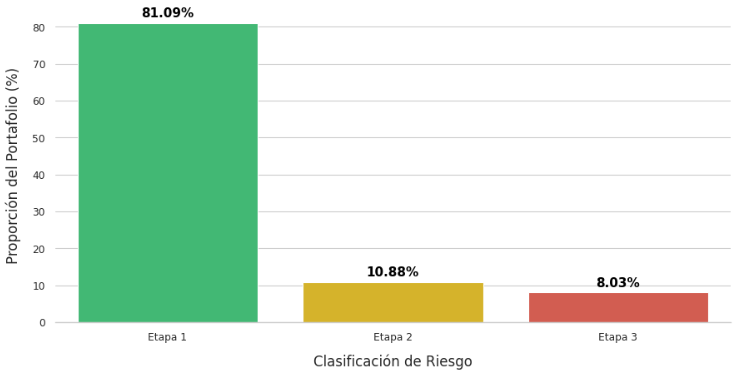
\includegraphics[scale=0.6]{imagenes/Capturas/graph-4-1.png}
	\vspace{0pt}
	\caption{Distribución de la variable \texttt{etapa}}
	\vspace{0pt}
\end{figure}

Esta distribución es esperable con la realidad del sector financiero; es indispensable para la viabilidad de las instituciones que la inmensa mayoría de la cartera se mantenga con un riesgo bajo, aplicando rigurosos filtros para evitar pérdidas. No obstante, un 18.91\% combinado de cartera con deterioro (Etapas 2 y 3) representa un volumen considerable crítico.
Esta proporción confirma la presencia de un \textit{desbalance de clases}. En consecuencia, la métrica de Exactitud (\textit{Accuracy}) queda descartada como criterio principal de evaluación. Un modelo predictivo ingenuo que clasificara a todas las cohortes en Etapa 1 obtendría un 81\% de exactitud, lo cual sería financieramente desastroso. Para la toma de decisiones institucionales, el costo de un Falso Negativo (evaluar una cohorte de alto riesgo como si fuera de riesgo bajo) es asimétricamente superior al de un Falso Positivo. Por tanto, el diseño de la red neuronal deberá priorizar la optimización de la Sensibilidad (\textit{Recall}) para la detección temprana de la cartera deteriorada.

\subsubsection{Distribución de las variables Financieras}
Las distribuciones de las masas monetarias muestran una alta asimetría positiva (\textit{Right Skewness}). Por ejemplo, el 75\% de las cohortes presentan un \texttt{monto\_originacion\_credito} igual o inferior a los \$4.2 millones de MXN; sin embargo, el límite superior alcanza cifras extremas de hasta \$3,151 millones de MXN. Como vimos en la detección de outliers, estas brechas gigantescas no constituyen errores, sino que reflejan realidades comerciales validas: cohortes masivas de miles de instrumentos hipotecarios o financiamientos de grandes desarrollos estructurales.  Por lo tanto, para una mejor visualización (sin el efecto visual de los outliers), se grafican las distribuciones en escala logarítmica.

Por otro lado, la \texttt{tasa\_ponderada} es la única variable que mantiene una estructura interpretable en escala lineal, con una media nacional del 10.31\% y una desviación estándar moderada del 1.91\%, presentando casos atípicos puntuales que escalan hasta el 36\% para esquemas de alto riesgo.

\begin{figure}[H]
	\centering
	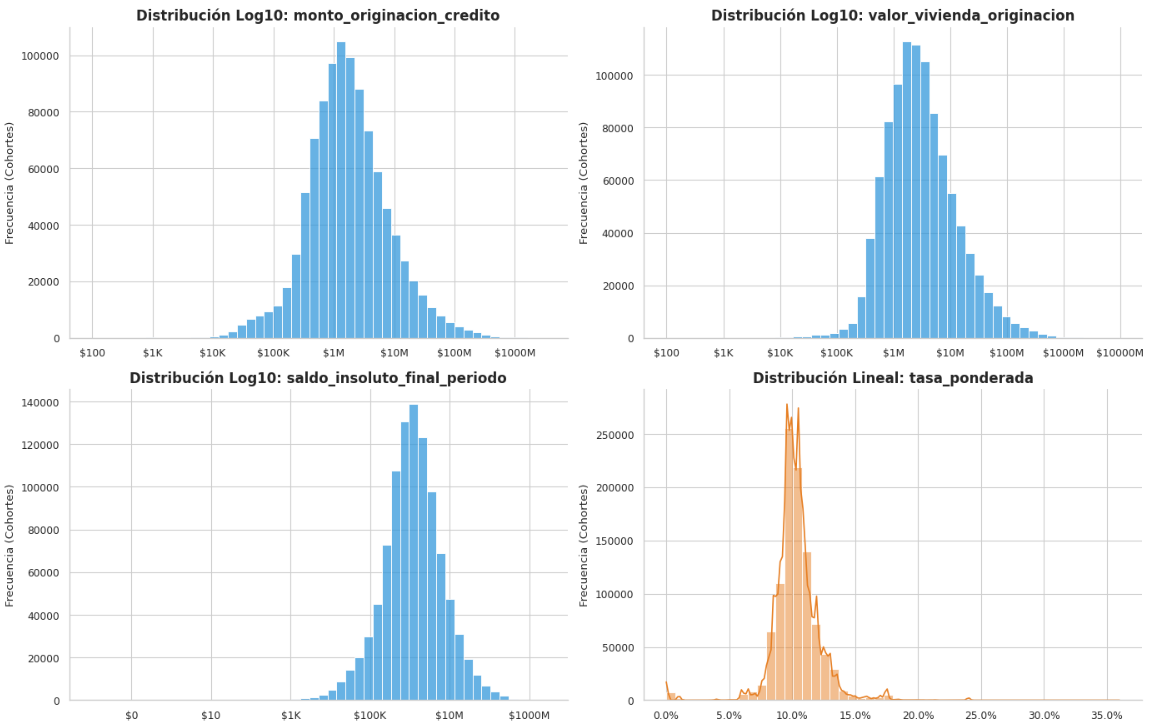
\includegraphics[scale=0.42]{imagenes/Capturas/graph-4-2.png}
	\vspace{0pt}
	\caption{Distribución de las variables financieras}
	\vspace{0pt}
\end{figure}

Para mitigar el efecto que estos valores extremos podrían inducir en los algoritmos sensibles a outliers, se corrobora la necesidad de aplicar transformaciones no lineales, como la transformación logarítmica o escaladores en la fase de preprocesamiento.

\subsubsection{Distribución de variables demográficas y socio-económicas}
El análisis de frecuencias de las variables categóricas revela una marcada concentración del portafolio en nichos poblacionales específicos:
\begin{itemize}
	\item Existe una concentración en los intervalos de edad de 36 a 45 años y de 46 a 55 años. Esto indica que el financiamiento hipotecario ocurre predominantemente en la mediana edad.
	\item Las cohortes financiadas se agrupan en los rangos de ingresos mensuales de \$20,001 a \$40,000 MXN y de \$40,001 a \$80,000 MXN. Esto evidencia que el mercado atiende principalmente a la clase media y media-alta.
	\item Una gran mayoría de las cohortes pertenece al Sector Privado (asalariados). Se identificó que las variables \texttt{tipo\_acreditado} y \texttt{sector\_laboral} proveen información redundante, justificando la eliminación de la primera para optimizar el espacio vectorial.
\end{itemize}

\begin{figure}[H]
	\centering
	\vspace{-10pt}
	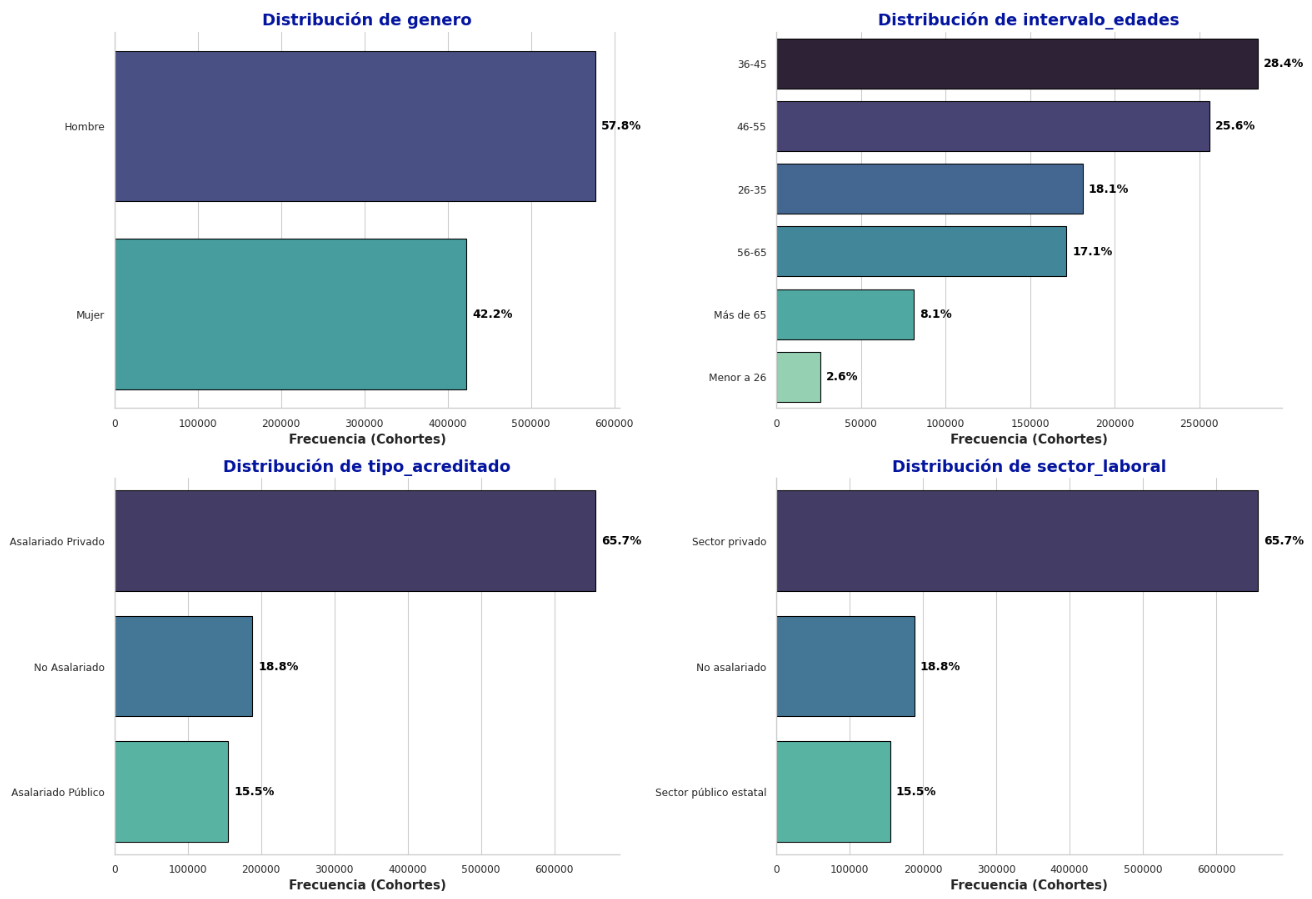
\includegraphics[scale=0.37]{imagenes/Capturas/graph-4-3.png}
	\vspace{-20pt}
\end{figure}
\begin{figure}[H]
	\centering
	\vspace{-10pt}
	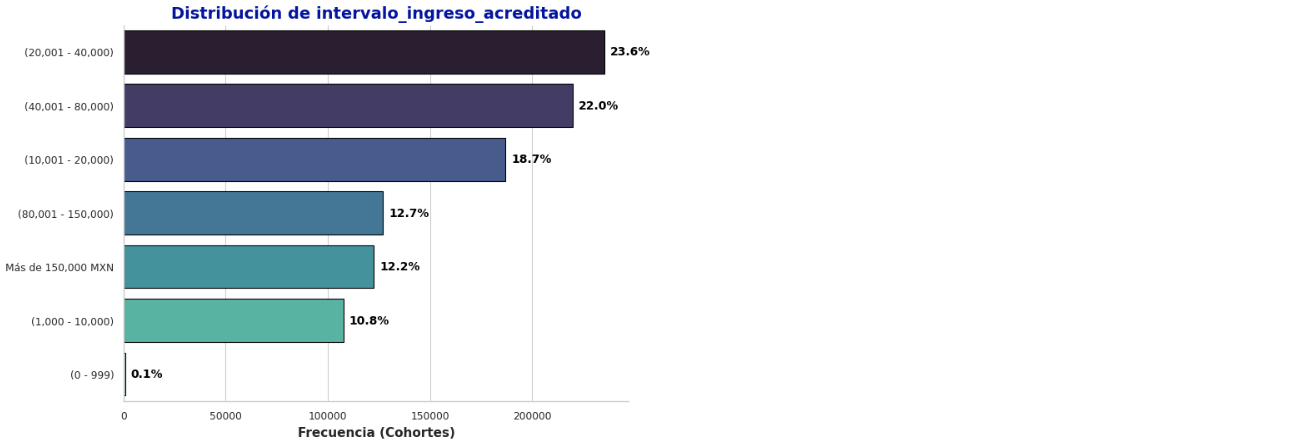
\includegraphics[scale=0.38]{imagenes/Capturas/graph-4-4.png}
	\caption{Distribución de las variables demográficas y socio-económicas}
	\vspace{-40pt}
\end{figure}

\subsubsection{Distribución de variables comerciales}
La naturaleza del activo en garantía y su localización geográfica también forman parte importante para alimentar a los modelos.
\begin{itemize}
	\item El crédito se centraliza en las regiones de mayor desarrollo industrial y económico del país: Ciudad de México (6.7\%), Jalisco (7.5\%) y Nuevo León (6.1\%).
	\item El portafolio se orienta fuertemente hacia la Adquisición de Vivienda Nueva (41.6\%) por encima de la vivienda usada (28.0\%). Asimismo, el 86.1\% de las cohortes se concentra en el segmento habitacional de nivel Medio o Residencial.
	\item La variable del nombre comercial del producto hipotecario exhibió una cardinalidad extrema (471 clases distintas), donde los 5 principales productos apenas consolidan el 21.95\% de la muestra. Esta fragmentación nos permite validar su exclusión del modelado predictivo al carecer de capacidad de generalización.
\end{itemize}

\subsubsection{Distribución de variables temporales e institucionales}
\begin{table}[H]
	\centering
	
	% Primera fila
	\begin{subtable}[t]{0.48\textwidth}
		\centering
		\caption{Periodo}
		\begin{tabular}{lrr}
			\toprule
			\textbf{Periodo} & \textbf{Frecuencia} & \textbf{\%} \\
			\midrule
			202504 & 40\,676 & 4.07 \\
			202411 & 40\,555 & 4.06 \\
			202502 & 40\,290 & 4.03 \\
			202508 & 40\,261 & 4.03 \\
			202506 & 40\,209 & 4.02 \\
			\vdots & \vdots & \vdots \\
			\bottomrule
		\end{tabular}
	\end{subtable}
	\hfill
	\begin{subtable}[t]{0.48\textwidth}
		\centering
		\caption{Sector}
		\begin{tabular}{lrr}
			\toprule
			\textbf{Sector} & \textbf{Frecuencia} & \textbf{\%} \\
			\midrule
			Banca Múltiple & 974\,696 & 97.47 \\
			Banca de Desarrollo & 16\,199 & 1.62 \\
			SOFOMER & 9\,105 & 0.91 \\
			\vdots & \vdots & \vdots \\
			\bottomrule
		\end{tabular}
	\end{subtable}
	
	\vspace{0.5cm}
	
	% Segunda fila
	\begin{subtable}[t]{0.48\textwidth}
		\centering
		\caption{Institución}
		\begin{tabular}{lrr}
			\toprule
			\textbf{Institución} & \textbf{Frecuencia} & \textbf{\%} \\
			\midrule
			Santander & 313\,014 & 31.30 \\
			Banorte & 187\,162 & 18.72 \\
			BBVA México & 155\,475 & 15.55 \\
			Scotiabank & 76\,672 & 7.67 \\
			HSBC & 75\,329 & 7.53 \\
			\vdots & \vdots & \vdots \\
			\bottomrule
		\end{tabular}
	\end{subtable}
	\hfill
	\begin{subtable}[t]{0.48\textwidth}
		\centering
		\caption{Moneda}
		\begin{tabular}{p{4.5cm} r r}
			\toprule
			\textbf{Moneda} & \textbf{Frecuencia} & \textbf{\%} \\
			\midrule
			Moneda Nacional (Pesos) & 978\,237 & 97.82 \\
			UDIS & 16\,303 & 1.63 \\
			VSMG (Veces Salario Mínimo General) & 5\,131 & 0.51 \\
			Dólares de E.E.U.U.A. & 329 & 0.03 \\
			\bottomrule
		\end{tabular}
	\end{subtable}
	\caption{Frecuencias de variables temporales e institucionales}
	
\end{table}
La distribución temporal resultó ser uniforme (aproximadamente un 4\% de los registros por cada mes reportado). Se explorará mejor en el análisis bivariado.

A nivel institucional, la Banca Múltiple consolida el 97.47\% de la cartera. Más aún, tan solo cinco instituciones acaparan más del 80\% de las cohortes hipotecarias a nivel nacional, lo que implica que las políticas de evaluación de estas entidades dictan la salud del mercado hipotecario. 

Finalmente, aunque el Peso Mexicano ejerce una hegemonía absoluta (97.82\%) sobre las demás divisas, estas otras divisas con volumen minoritario serán de importancia en el análisis bivariado.

% ============================================================

\subsection{Análisis Bivariado}

Tras estudiar el comportamiento individual de las variables, la segunda fase del Análisis Exploratorio de Datos consistió en evaluar las relaciones entre dos categorías, en particular su impacto directo sobre la variable objetivo. El propósito es identificar los predictores más robustos del deterioro crediticio y descartar aquellos que inyectan redundancia matemática al sistema.

\subsubsection{Correlación y Colinealidad en Variables Financieras}
En el modelado supervisado, la inclusión de atributos altamente correlacionados genera inestabilidad en los gradientes y aumenta innecesariamente el costo computacional. Para evaluar esta métrica, se calculó una matriz de correlación de Pearson sobre las variables monetarias continuas.

Los resultados confirmaron una colinealidad extrema ($|r| > 0.90$) entre la gran mayoría de las métricas de volumen. Por ejemplo, el coeficiente de correlación entre el saldo insoluto final y la masa de intereses generados alcanzó un 0.999. Paralelamente, el monto de originación del crédito y el valor de la vivienda presentaron un coeficiente de 0.949. Por consiguiente, esta exploración justifica la decisión de conservar exclusivamente el \texttt{saldo\_insoluto\_final\_periodo} como único indicador de volumen monetario y la \texttt{tasa\_ponderada} como indicador del costo del dinero, dada su independencia lineal frente a las métricas de volumen.

\begin{figure}[H]
	\centering
	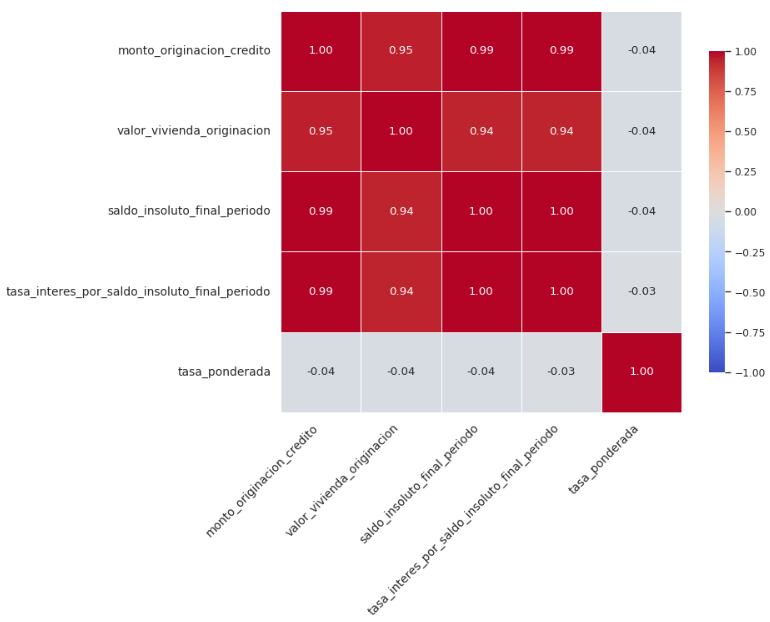
\includegraphics[scale=0.6]{imagenes/Capturas/graph-4-7.png}
	\vspace{0pt}
	\caption{Heatmap de correlación (Person) en variables financieras}
	\vspace{0pt}
\end{figure}

Al proyectar estas dos variables finales en diagramas de dispersión junto con una tercera dimensión de color (`etapa`), se evidenció la formación de nubes densas y bandas horizontales. Estas franjas reflejan la estandarización comercial de tasas fijas (del 9\%, 10.5\%, 11\%, etc.). La dispersión demostró que el riesgo no es linealmente separable mediante dos dimensiones continuas; las cohortes en Etapa 3 coexisten en los mismos rangos de tasa y saldo que las cohortes en Etapa 1, evidenciando que el incumplimiento es un fenómeno multidimensional.

\begin{figure}[H]
	\centering
	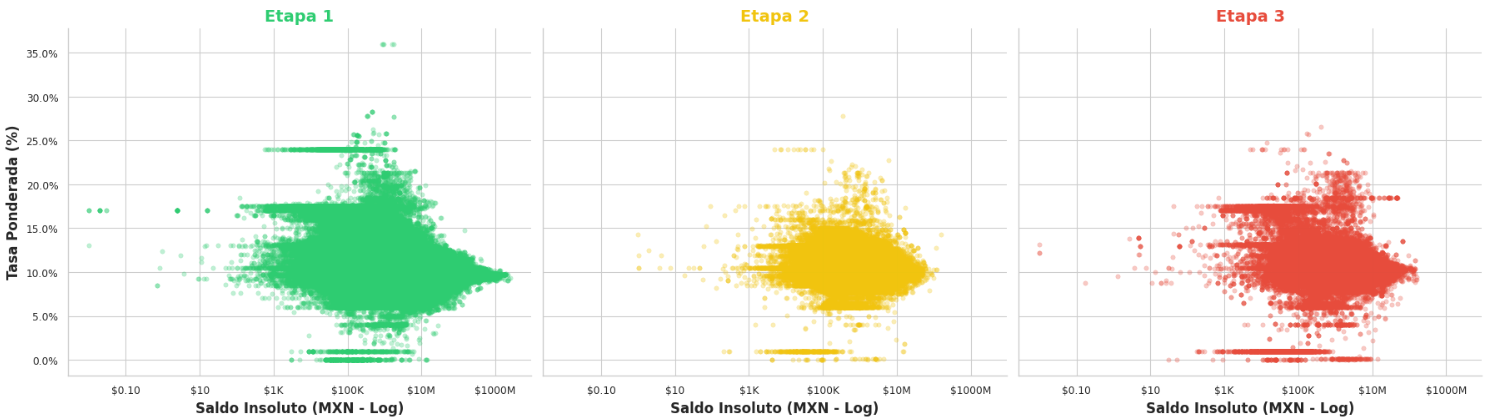
\includegraphics[scale=0.32]{imagenes/Capturas/graph-4-8.png}
	\vspace{0pt}
	\caption{Dispersión de saldo vs tasa de interés por etapas de riesgo}
	\vspace{0pt}
\end{figure}

\subsubsection{Dinámica de Riesgo: Variables catégoricas - Variable Objetivo}
Para cuantificar el impacto de los perfiles demográficos y comerciales sobre el riesgo, se definió la \textit{Tasa de Deterioro}. El Deterioro $D$ es la probabilidad condicional de que una cohorte transite hacia el riesgo significativo o alto $Y \in\{ \text{``Etapa 2''} \cup \text{``Etapa 3''}\}$, dado un atributo específico, $X = x_i$.:
$$
P(D \mid X = x_i) = \frac{\text{Frecuencia}(Y \in \{2,3\} \cap X = x_i)}{\text{Frecuencia}(X = x_i)}
$$
Calcular $P(D \mid X)$ nos permite identificar si una variable es útil para nuestro futuro modelo. Si la probabilidad de deterioro es demasiado similar en todas las categorías de $X$ (ej. hombres y mujeres incumplen exactamente igual), la variable no aporta información discriminante. Si la probabilidad cambia drásticamente, hemos encontrado un fuerte predictor de riesgo.

Se encontraron los siguientes hallazgos:
\begin{itemize}
	\item Los esquemas UDIS (28.18\% de deterioro) y Veces Salario Mínimo General o VSMG (29.37\%) exhiben tasas de incumplimiento muy superiores a las originaciones en Moneda Nacional (18.69\%), a pesar de que esta última predomina en las observaciones. Lo más destacado es que las obligaciones en Dólares presentaron la mayor tasa de deterioro (42.25\%), evidenciando se debe mantener a la divisa para evitar introducir sesgos en el entrenamiento.
	\item Las cohortes integradas por empleados del sector público poseen el riesgo más bajo del portafolio (10.83\%), en contraste con el sector privado (21.83\%).
	\item El riesgo de incumplimiento respecto a la edad no es lineal. Se concentra de manera acentuada en la adultez joven y madura: 36-45 años con un 21.73\% de deterioro, 26-35 años con 20.55\%, y 46-55 con 20.41\%, mientras que otros sectores más jovenes o en edad de vejez tienen una tasa aproximada de 14\%.
	\item Contrario a la intuición de una relación inversa (quien gana más está menos endeudado), la dinámica de ingreso-riesgo no es lineal. Los estratos medios-altos (ingresos de \$40,001 a \$150,000 MXN) resultaron ser los de menor riesgo (aprox 17\%). Los de mayores ingresos ("Más de \$150,000 MXN") y menos ingresos (10,001 - 20,000)  presentaron las más altas tasas de deterioro (21.21\%), aunque no hay que perder de vista qu esto puede sugiere un alto apalancamiento relativo en propiedades de inversión o de lujo (para los primeros), o bien, una gran densidad de individuos agrupados en una misma coherte (para los segundos).
	\item La adquisición de vivienda usada conlleva un riesgo de incumplimiento manifiestamente mayor (25.18\%) frente a la vivienda nueva (19.15\%). Esto puede estar asociado a imprevistos estructurales y costos de mantenimiento que comprometen la liquidez de los acreditados.
\end{itemize}

% [recordatorio para insertar gráficas de barra de la tasa de deterioro]

\subsubsection{Dinámica de Riesgo: Variables continuas - Variable Objetivo}
Al analizar la interacción entre las variables continuas y las etapas de riesgo mediante diagramas de caja (\textit{Boxplots}), se mostraron asimetrías importantes.

La mediana de los montos de originación para las cohortes de riesgo bajo (Etapa 1) es significativamente superior (\$1.7M) a la de las cohortes con deterioro o en incumplimiento (aprox \$1M). Como se explicó antes, el segmento de Interés Social (asociado a montos menores) aporta mayores tasas de incumplimiento que los montos mayores, ya que estos créditos exigen filtros más estrictos para evitar pérdidas severas para las instituciones, reduciendo su probabilidad de impago.

Por su parte, la mediana de la tasa ponderada asciende de forma suave conforme crece el nivel de riesgo (del 10.10\% en Etapa 1 al 10.50\% en Etapa 3). Este diferencial, aunque pequeño, indica que las instituciones logran identificar e manejar el riesgo relativo desde la originación, penalizando a las cohortes moroso con un costo de capital ligeramente superior (tampoco se pretende castigar excesivamente, para evitar agravar aún más la deuda).

\begin{figure}[H]
	\centering
	\vspace{-10pt}
	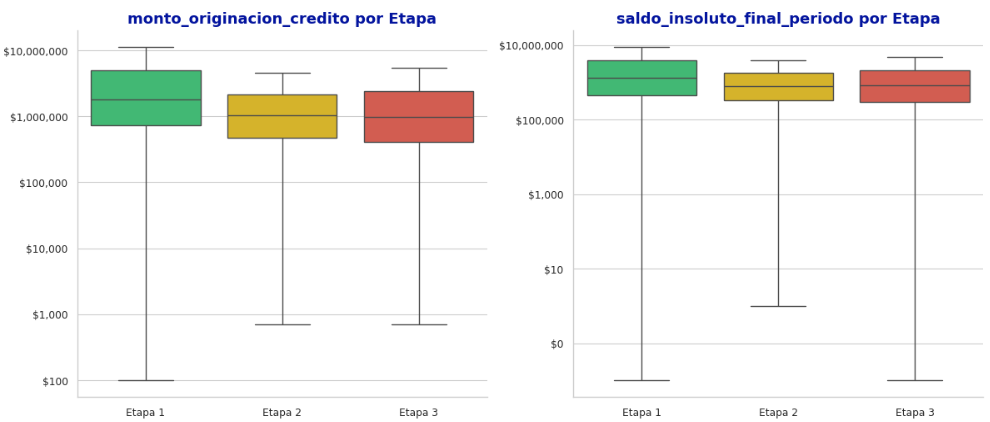
\includegraphics[scale=0.39]{imagenes/Capturas/graph-4-9.png}
	\vspace{-20pt}
\end{figure}
\begin{figure}[H]
	\centering
	\vspace{0pt}
	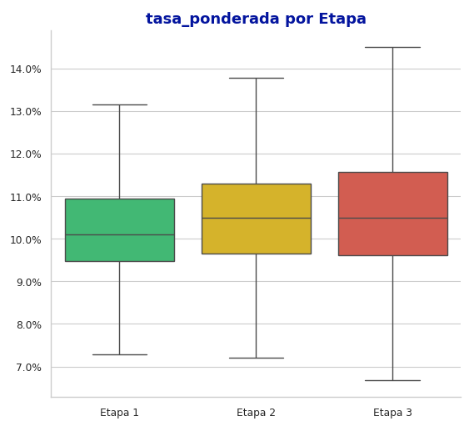
\includegraphics[scale=0.4]{imagenes/Capturas/graph-4-10.png}
	\caption{Boxplots de las variables financieras por etapas de riesgo}
	\vspace{-10pt}
\end{figure}

\subsubsection{Visualizaciones adicionales con Series de Tiempo}
El riesgo crediticio es un sujeto al tiempo, debido a las políticas monetarias y la pérdida de poder adquisitivo. Para concluir el análisis, se evaluó la evolución histórica de la Tasa de Deterioro a lo largo de los 25 meses disponibles en la muestra.

La serie de tiempo reveló una tendencia de deterioro gradual pero sostenida en el portafolio. En abril de 2024, el riesgo acumulado de las Etapas 2 y 3 se ubicaba en 18.28\%. Durante los siguientes 24 meses, la métrica experimentó un incremento escalonado hasta alcanzar un pico de 19.52\% a finales de 2025, estabilizándose en 19.36\% para el cierre del último mes reportado en abril de 2026. 

\begin{figure}[H]
	\centering
	\vspace{-10pt}
	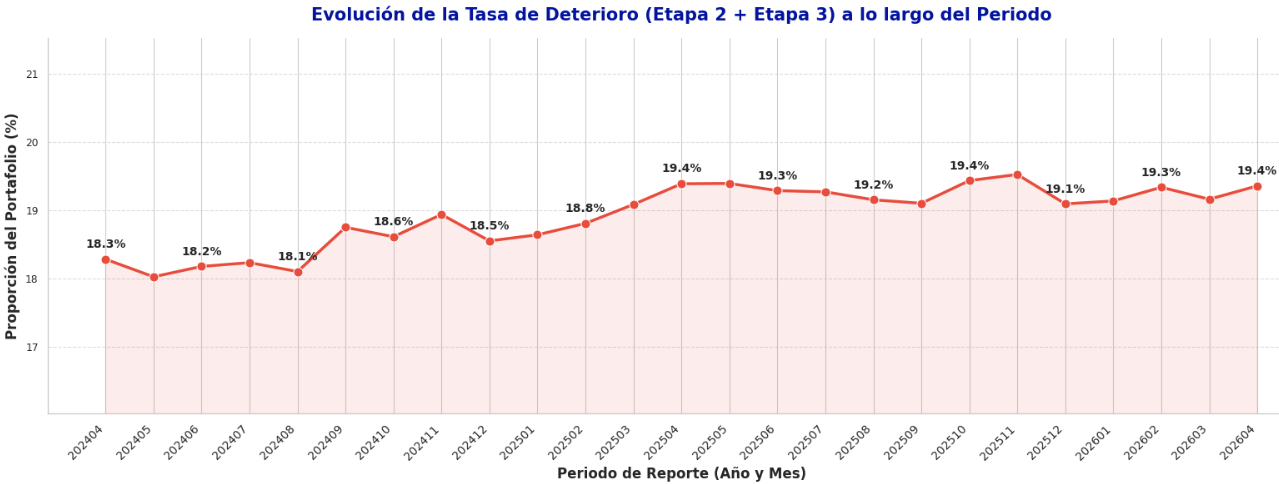
\includegraphics[scale=0.38]{imagenes/Capturas/graph-4-11.png}
	\caption{Serie de Tiempo de la Tasa de Deterioro}
	\vspace{-10pt}
\end{figure}

\subsection{Conclusiones y Selección de Características}
Concluida la exploración univariada y bivariada, se posee un entendimiento riguroso de las distribuciones y relaciones subyacentes en el conjunto de datos. Esto fue de vital importancia para justificar las decisiones presentadas en la sección \text{3.5. Reducción de Dimensionalidad y Selección de Características}.

Por lo que tras todo este proceso analítico, la dimensionalidad original de 20 columnas se redujo a un vector más manejable y altamente interpretable de 10 atributos esenciales: 
\begin{table}[H]
	\centering
	\begin{tabular}{r p{7cm} l}
		\hline
		& \textbf{Variable} & \textbf{Tipo de variable} \\
		\hline
		0 & \texttt{intervalo\_edades} & Categórica ordinal \\
		1 & \texttt{intervalo\_ingreso\_acreditado} & Categórica ordinal \\
		2 & \texttt{sector\_laboral} & Categórica nominal \\
		3 & \texttt{estado} & Categórica nominal \\
		4 & \texttt{destino\_credito} & Categórica nominal \\
		5 & \texttt{segmento\_vivienda} & Categórica nominal \\
		6 & \texttt{moneda} & Categórica nominal \\
		7 & \texttt{saldo\_insoluto\_final\_periodo} & Numérica continua \\
		8 & \texttt{tasa\_ponderada} & Numérica continua \\
		9 & \texttt{etapa} & Categórica ordinal \\
		\hline
	\end{tabular}
\end{table}

    \section{Modelo Supervisado}

Se modeló un algoritmo de aprendizaje automático capaz de aprender los patrones históricos de la cartera y predecir la probabilidad de que una nueva cohorte transite hacia el deterioro. El problema se define matemáticamente como una tarea de clasificación multiclase, donde se busca estimar la probabilidad condicional $P(Y=k \mid X=x^{(i)})$, siendo $X$ el vector de características de 10 dimensiones reducido en el capítulo anterior, y $Y \in \{1, 2, 3\}$ el espacio correspondiente a las etapas de riesgo definidas por la NIFBdM C-16.

\subsection{Estrategia de Evaluación y Desbalance de Clases}
El análisis exploratorio confirmó un desbalance de clases severo: la Etapa 1 (riesgo bajo) agrupa aproximadamente el 81\% de la muestra. Bajo esta asimetría, utilizar la Exactitud (\textit{Accuracy}) como métrica de éxito resulta engañoso; un clasificador trivial alcanzaría un 81\% de exactitud simplemente asignando a todas las cohortes la categoría de riesgo bajo.

Para las instituciones financieras, el costo de un Falso Negativo (clasificar una cartera altamente riesgosa como una de riesgo bajo) es por mucho, superior al de un Falso Positivo (sobreestimar el riesgo de una cohorte). Por consiguiente, la evaluación del modelo priorizarán la métrica de \textbf{Sensibilidad (\textit{Recall})} para las Etapas 2 y 3, garantizando la detección temprana del deterioro estructural, aun si esto implica un decremento en la Precisión (\textit{Precision}). Adicionalmente, se utilizará el Área Bajo la Curva ROC (AUC) para medir la capacidad de separación matemática entre clases.

\subsection{Preprocesamiento y Partición de Datos}
Se aplicó un muestreo aleatorio estratificado, dividiendo los datos en tres subconjuntos: Entrenamiento (64\%), Validación (16\%) y Prueba (20\%). 

Posteriormente, se aplicaron transformaciones matemáticas calibradas exclusivamente sobre el conjunto de entrenamiento:
\begin{itemize}
	\item \textbf{Variables Continuas:} Se utilizó un escalamiento (\textit{RobustScaler}), el cual sustrae la mediana y divide por el rango intercuartílico, protegiendo los gradientes contra la extrema asimetría de las magnitudes monetarias.
	\item \textbf{Variables Categóricas:} Se le aplicó codificación \textit{One-Hot}, expandiendo la dimensionalidad de entrada a un vector final de 71 dimensiones ($d=71$).
\end{itemize}

Para abordar el desbalance, se calculó un vector de pesos inversamente proporcional a las frecuencias de clase. Este vector penaliza los errores matemáticos cometidos sobre la clase minoritaria. Matemáticamente, el modelo penaliza aproximadamente 10 veces más un error de clasificación en la Etapa 3 que en la Etapa 1 (esto para evitar al máximo, los Falsos Positivos).

\subsection{Línea Base: Regresión Logística Multiclase}
Para establecer un umbral de desempeño, se entrenó un modelo estadístico lineal de Regresión Logística. Los resultados reflejaron las limitaciones de los modelos lineales ante dinámicas financieras complejas. A pesar de incorporar los pesos compensatorios, el modelo apenas logró un \textit{Recall} del 42\% para la Etapa 3. Las fronteras del riesgo demostraron no ser linealmente separables, haciendo necesario la transición hacia modelos no lineales.

\subsection{Arquitectura de la Red Neuronal Multicapa (MLP)}
Se seleccionó el \textit{framework} PyTorch para implementar una Red Neuronal Profunda, dada su escalabilidad y la flexibilidad para manipular directamente la función de pérdida. La arquitectura diseñada consta de:
\begin{enumerate}
	\item \textbf{Capa de Entrada:} El vector multidimensional ($X \in \mathbb{R}^{71}$).
	\item \textbf{Capas Ocultas:} Dos capas secuenciales (128 y 64 neuronas) con funciones de activación no lineales ReLU (\textit{Rectified Linear Unit}).
	\item \textbf{Regularización:} Para evitar el sobreajuste (\textit{overfitting}), se intercalaron capas de \textit{Dropout} con una probabilidad de apagado neuronal del 30\%.
	\item \textbf{Capa de Salida y Optimización:} Un vector de tres dimensiones que representa cada etapa de riesgo.
\end{enumerate}
Además, para cuantificar el error en cada etapa, para la función de pérdida usamos Entropía Cruzada Categórica, la cuál internaliza los pesos de desbalance, y como optimizador el algoritmo Adam.

El ciclo de aprendizaje se ejecutó mediante descenso de gradiente por mini-lotes (\textit{Mini-Batch Gradient Descent}). El monitoreo de la pérdida, demostró la ausencia de sobreajuste: la pérdida del conjunto de validación descendió simétricamente a la pérdida de entrenamiento durante 30 épocas, logrando una convergencia altamente estable.

\begin{table}[H]
	\centering
	\begin{tabular}{rcc}
		\hline
		\textbf{Época} & \textbf{Train Loss} & \textbf{Validation Loss} \\
		\hline
		01/30 & 0.9798 & 0.9512 \\
		02/30 & 0.9508 & 0.9383 \\
		03/30 & 0.9421 & 0.9313 \\
		04/30 & 0.9356 & 0.9259 \\
		05/30 & 0.9313 & 0.9247 \\
		\vdots & \vdots & \vdots \\
		25/30 & 0.9098 & 0.9060 \\
		26/30 & 0.9088 & 0.9064 \\
		27/30 & 0.9088 & 0.9058 \\
		28/30 & 0.9082 & 0.9043 \\
		29/30 & 0.9082 & 0.9056 \\
		30/30 & 0.9078 & 0.9053 \\
		\hline
	\end{tabular}
\end{table}

\subsection{Evaluación Final e Interpretación}
La red neuronal fue evaluada de manera definitiva sobre los 200,000 registros del conjunto de prueba, revelando una capacidad de generalización notablemente superior a la \textit{linebase}.

\subsubsection{Mejora de Sensibilidad}
El MLP incrementó el \textit{Recall} de la Etapa 3 hasta un 52\% (frente al 42\% del modelo lineal) y el de la Etapa 2 hasta un 62\%. Esto significa que la red identificó proactivamente más de 1,600 cohortes deterioradas adicionales que el modelo lineal había omitido. Considerando la magnitud monetaria del portafolio, esta mejora se traduce en la detección temprana de miles de millones de pesos en riesgo de impago.

\begin{figure}[H]
	\centering
	\vspace{-10pt}
	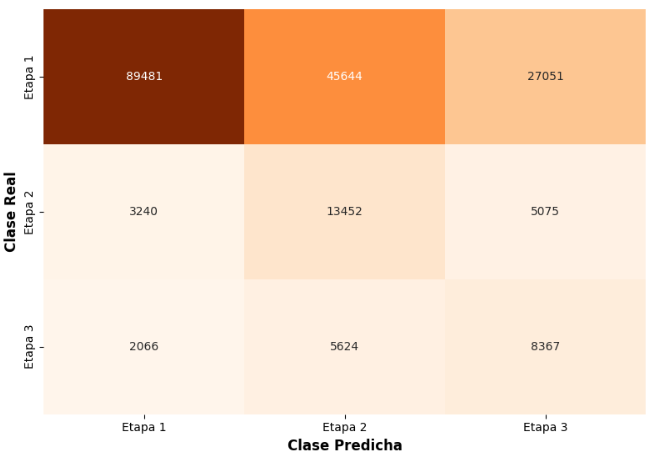
\includegraphics[scale=0.43]{imagenes/Capturas/graph-5-1.png}
	\caption{Matriz de Confusión Multiclase (Red Neuronal)}
	\vspace{-20pt}
\end{figure}

Como contraparte, la Precisión (\textit{Precision}) para las clases de riesgo se situó en un 21\%. Es decir, de cada cinco cohortes alertadas por el sistema, cuatro corresponden a un riesgo bajo. No obstante, desde la perspectiva de la gestión de riesgo, esto representa la estrategia de la que hablamos previamente: es preferible asumir los costos de pérdida de los Falsos Positivos, que absorber la pérdida total del capital por un incumplimiento no anticipado (Falsos Negativos).

\subsubsection{Curva ROC y Área Bajo la Curva (AUC)}
Para visualizar el desempeño discriminativo del modelo, se analizaron las curvas ROC bajo un esquema uno-contra-todos. La red neuronal alcanzó un AUC unificado y estable en el espectro de riesgo: 0.79 (Etapa 1), 0.76 (Etapa 2) y 0.78 (Etapa 3). 

\begin{figure}[H]
	\centering
	\vspace{0pt}
	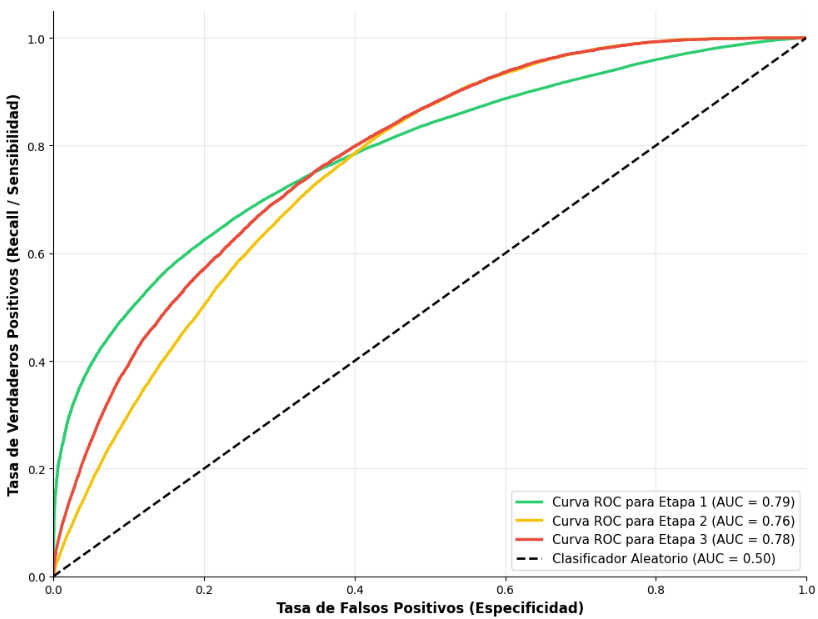
\includegraphics[scale=0.45]{imagenes/Capturas/graph-5-2.png}
	\caption{Curvas ROC Multiclase (One-vs-Rest)}
	\vspace{-10pt}
\end{figure}

Un AUC de 0.78 en la cartera deteriorada confirma que el modelo posee un 78\% de probabilidad de asignar un mayor puntaje de riesgo a una cohorte estadísticamente vulnerable frente a una cohorte estable. Lograr este grado de separación únicamente a través de demografía estática y características comerciales (sin consultar inflación o temporalidad) demuestra una alta eficacia de la arquitectura para la predicción de nuevas observaciones.




    \section{Clustering}
El propósito en esta fase no es anticipar una etiqueta conocida, sino descubrir la estructura intrínseca y los patrones ocultos que residen en la base de datos. 

\subsection{Definición del Enfoque y Submuestreo}
Aplicar un algoritmo de agrupamiento sobre el total de la muestra (1,000,000 de registros) resultaría computacionalmente ineficiente e irrelevante para el negocio. Se adoptó la decisión de **aislar y analizar de manera exclusiva la cartera en Etapa 3 (Riesgo Alto)**. Esto se sustenten en que el incumplimiento no es un fenómeno homogéneo; las cohortes transitan hacia la cartera vencida impulsadas por diferentes combinaciones de vulnerabilidades demográficas, socioeconómicas y estructurales. Al agrupar únicamente a las observaciones deterioradas, el algoritmo responderá a una pregunta: \textit{¿Cuáles son los perfiles estructurales del incumplimiento hipotecario en México?}

A partir de la muestra de un millón de registros, de las 80,285 cohortes clasificadas en Etapa 3 (obtenidas por la partición del modelo supervisado para el conjunto de pruebas), para garantizar la viabilidad computacional en el cálculo de distancias cruzadas, se extrajo una submuestra aleatoria representativa de 10,000 registros, excluyendo la variable constante \texttt{etapa} (ya que toda esta muestra es de la Etapa 3) resultando en un vector de 9 dimensiones.

\subsubsection{Métrica de Similitud: Distancia de Gower}
La \textit{Distancia Euclidiana} es inapropiada para datos categóricos . Para solucionar esto, se implementó la \textbf{Distancia de Gower}. Esta métrica calcula una similitud parcial dependiendo de la naturaleza de cada variable: para las métricas financieras calcula diferencias absolutas estandarizadas por el rango máximo, para mitigar los atípicos; para las dimensiones categóricas, aplica un coeficiente de coincidencia binaria. La agregación de estas similitudes genera una matriz cuadrada $(10,000 \times 10,000)$ donde los valores oscilan estrictamente entre $0$ (cohortes idénticas) y $1$ (cohortes diametralmente opuestas).

\subsubsection{Algoritmo de Particionamiento: PAM (K-Medoids)}
Evaluando las alternativas algorítmicas, \textit{K-Means} fue descartado debido a su alta sensibilidad a valores atípicos y a su incapacidad para generar centroides reales y fielmente interpretables en datos categóricos. 

En su lugar, se seleccionó el algoritmo \textbf{PAM (\textit{Partitioning Around Medoids})}. PAM opera minimizando la suma de distancias absolutas a un conjunto de observaciones representativas llamadas \textit{medoides}. Su ventaja radica en la robustez frente a extremos monetarios y, críticamente, en su interpretabilidad: el centroide de cada clúster no es un promedio, sino un registro real en la base de datos.

\subsection{Determinación de Clústeres y Validación Dimensional}
Para determinar el hiperparámetro $K$ (número de grupos), se ejecutó una validación interna utilizando el \textbf{Coeficiente de Silueta} sobre la matriz de Gower precomputada.

El coeficiente evaluó la cohesión interna y la separación externa de los grupos para valores desde $K=2$ hasta $K=6$. El rendimiento máximo se alcanzó en \textbf{$K=2$}.

\begin{figure}[H]
	\centering
	\vspace{-0pt}
	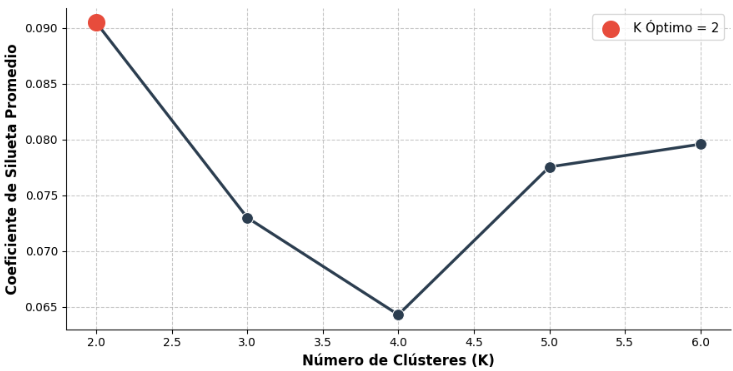
\includegraphics[scale=0.45]{imagenes/Capturas/graph-6-1.png}
	\caption{Coeficiente de Silueta evaluando distintos valores de $K$}
	\vspace{-10pt}
\end{figure}

Posterior a la partición por PAM, se aplicó una técnica de reducción de dimensionalidad no lineal, t-SNE (\textit{t-distributed Stochastic Neighbor Embedding}) a partir de la matriz de Gower para proyectar la separación de los clústeres en un espacio bidimensional, confirmando que el algoritmo logró separar la cartera vencida en dos nubes de densidad.

\begin{figure}[H]
	\centering
	\vspace{-0pt}
	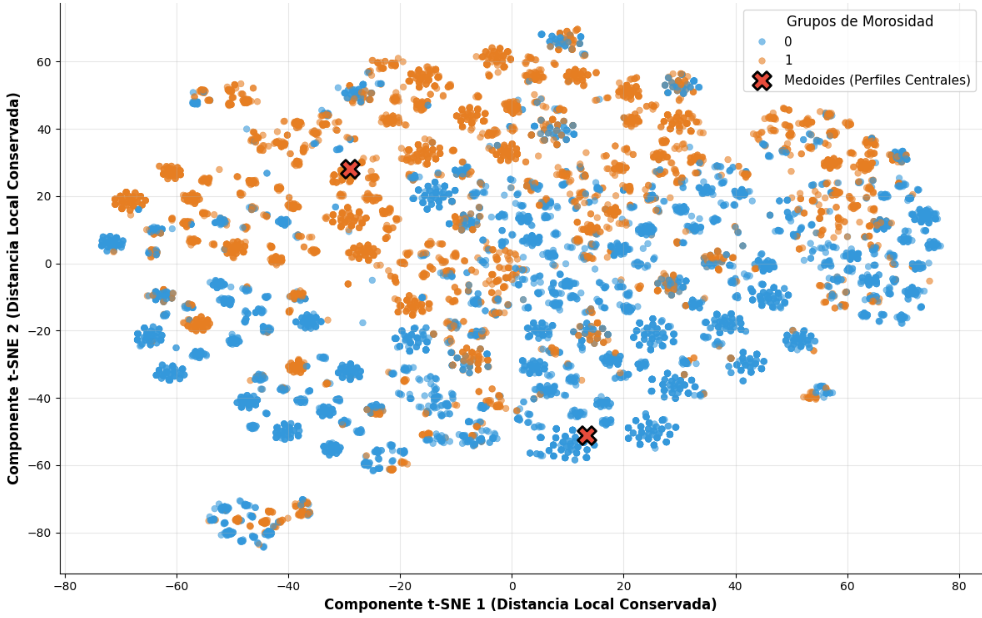
\includegraphics[scale=0.45]{imagenes/Capturas/graph-6-2.png}
	\caption{Proyección t-SNE bidimensional de los clústeres de la Etapa 3}
	\vspace{-10pt}
\end{figure}

\subsection{Interpretación de los Perfiles de Morosidad}
Para interpretar claramente los agrupamientos , se cruzaron las asignaciones del modelo PAM con el vector de características original.

Como primer análisis visual preliminar, mostrado mediante gráficos de dispersión estocástica (\textit{Stripplots}) entre edad e ingreso, insinuó patrones de agrupación en cuadrantes específicos de la matriz demográfica. Sin embargo, para cuantificar las fronteras de manera más completa e integra, se recurrió al análisis de frecuencias de las dimensiones categóricas estructurales.

\begin{figure}[H]
	\centering
	\vspace{-0pt}
	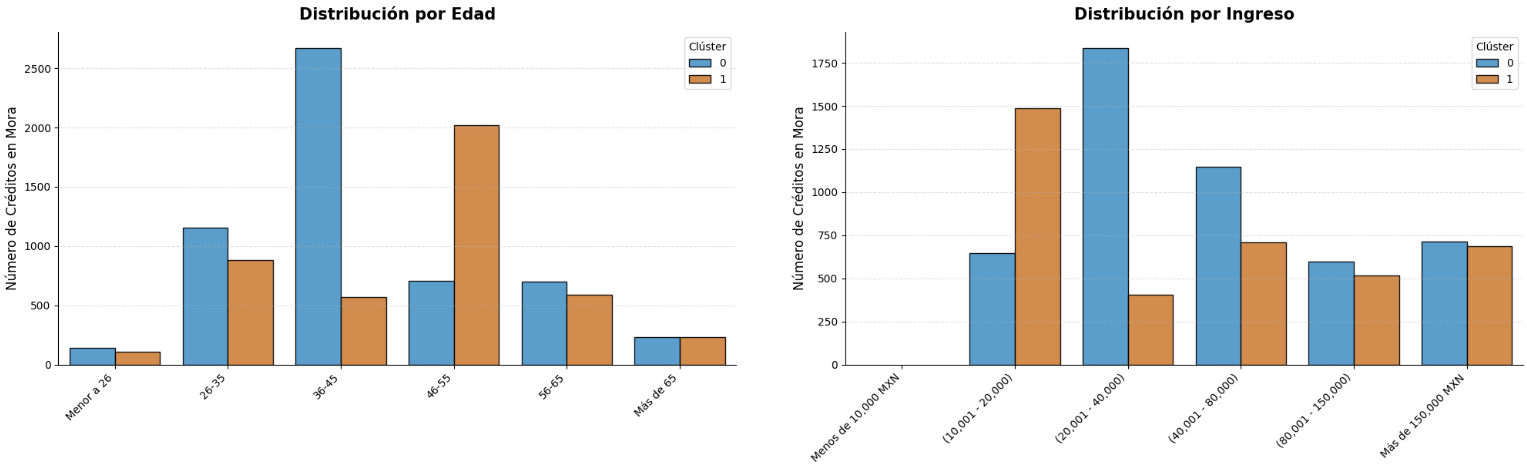
\includegraphics[scale=0.32]{imagenes/Capturas/graph-6-3.png}
	\vspace{-10pt}
\end{figure}
\begin{figure}[H]
	\centering
	\vspace{-0pt}
	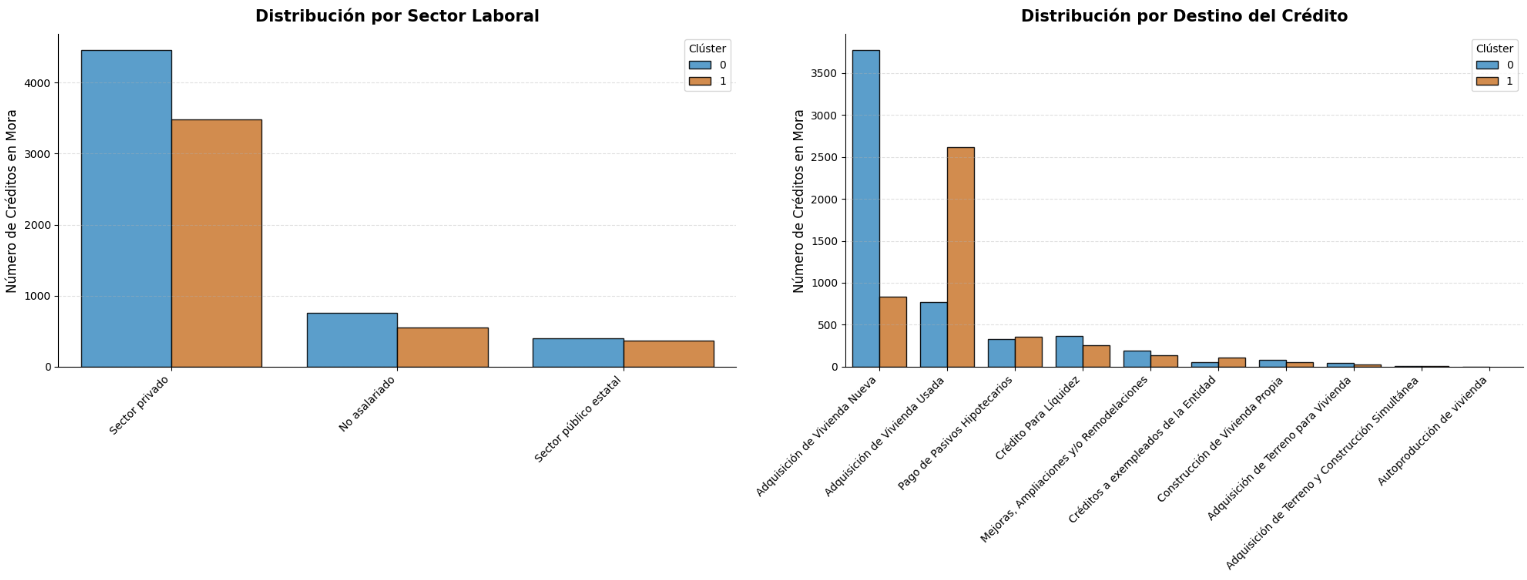
\includegraphics[scale=0.32]{imagenes/Capturas/graph-6-4.png}
	\vspace{-10pt}
\end{figure}
\begin{figure}[H]
	\centering
	\vspace{-0pt}
	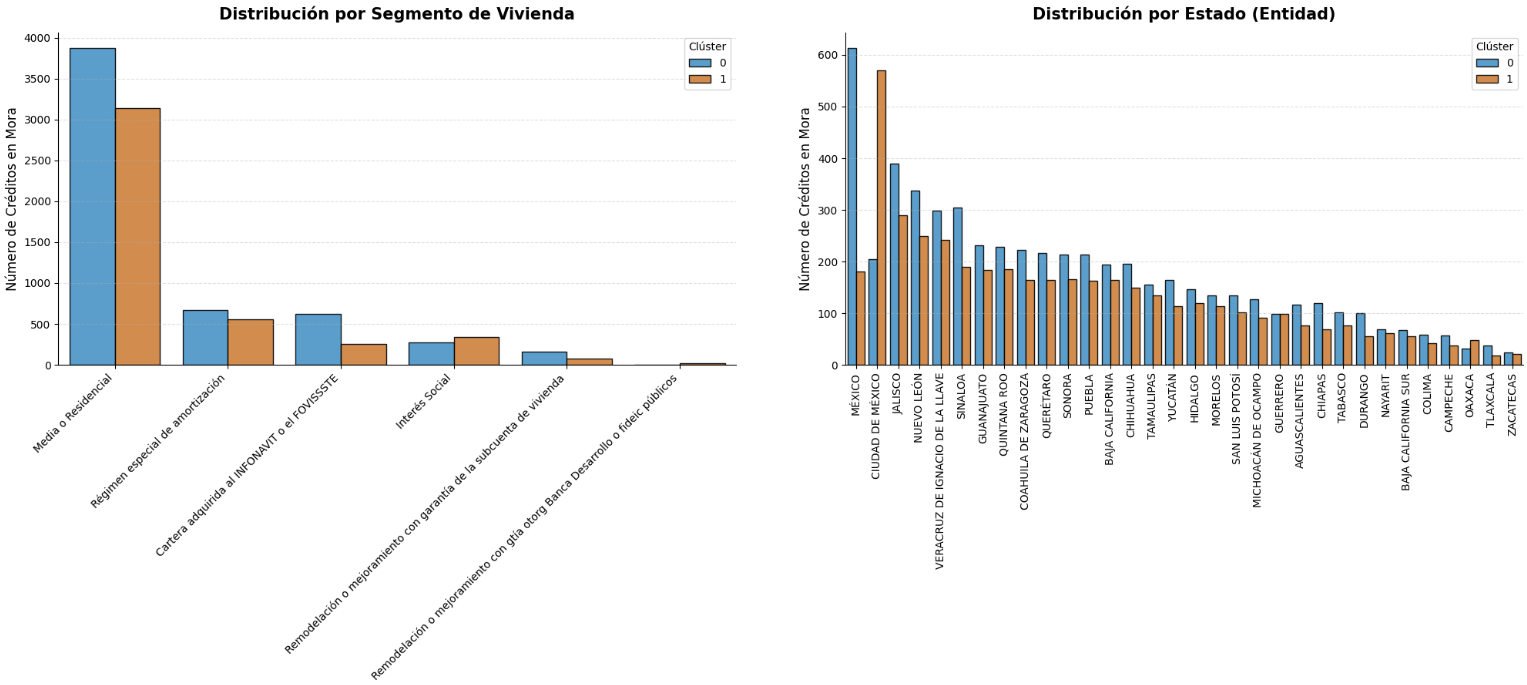
\includegraphics[scale=0.32]{imagenes/Capturas/graph-6-5.png}
	\caption{Distribución de los clústeres de la Etapa 3 en las variables catégoricas}
	\vspace{-10pt}
\end{figure}

La convergencia de estos análisis visuales con la identidad financiera de los medoides revelados por el algoritmo, reveló formalmente los dos principales perfiles que originan el deterioro crediticio:

\begin{itemize}
	\item \textbf{Perfil 0:} \\
	Agrupa a cohortes en una etapa de madurez media (36-45 años) con ingresos medios-altos (\$20,001 a \$40,000 MXN). El deterioro surge en operaciones destinadas a la \textit{Adquisición de Vivienda Nueva}, típicamente ubicadas en la periferia de crecimiento urbano continuo (como el Estado de México). Presentan deudas conjuntas moderadas (mediana cercana a los \$754,566 MXN) a tasas estandarizadas (10.75\%). 
	
	\item \textbf{Perfil 1:} \\
	Agrupa a cohortes en etapas de mayor madurez (46-55 años) y con una ingresos inferiores (\$10,001 a \$20,000 MXN). El incumplimiento en este estrato se acentúa en \textit{Adquisición de Vivienda Usada}, concentrándose fuertemente en el centro del país (Ciudad de México). Contraintuitivamente a sus ingresos, las cohortes de este grupo sostienen niveles de deuda conjuntas muy elevados (mediana superior a \$1.3 millones MXN) a tasas ligeramente preferenciales (10.00\%). 
\end{itemize}

\subsection{Conclusión del Análisis Descriptivo}
El modelo no supervisado dotó perfiló el concepto de riesgo alto. Mientras que las redes neuronales operan como predictores de riesgo, el agrupamiento con K-Medoids indentifico la estructura que toma la cartera vencida. Al revelar que las carteras deterioradas no son uniformes, las instituciones pueden implementar estrategias especializadas (por ejemplo, esquemas de refinanciamiento temporal para el Perfil 0, o apoyos para liquidaciones para el Perfil 1), optimizando las pérdidas y recuperando liquidez.
\end{spacing}

\nocite{*}

% \bibliographystyle{ACM-Reference-Format}
% \bibliography{contenido/referencias.bib}

\end{document}